%% Main File
%% 
%% This file uses the abnTex2 to compile a dissertation for the Programa 
%% de Pós-Graduação em Engenharia Elétrica da PUCRS.

\documentclass[
	% Options - memoir
	12pt,		% Font size
    openright, 	% Chapters start in odd page
    oneside,	% Bothsides printing
    a4paper,	% Paper size
    % Options - abntex2
   	%chapter=TITLE,		% títulos de capítulos convertidos em letras maiúsculas
	%section=TITLE,		% títulos de seções convertidos em letras maiúsculas
	%subsection=TITLE,	% títulos de subseções convertidos em letras maiúsculas
	%subsubsection=TITLE,% títulos de subsubseções convertidos em letras maiúsculas
	% -- opções do pacote babel --
	%english,			% idioma adicional para hifenização
	french,				% idioma adicional para hifenização
	spanish,			% idioma adicional para hifenização
	english,				% o último idioma é o principal do documento
    brazil,				% o último idioma é o principal do documento
]{abntex2}

% ---
% PACOTES
% ---


% ---
% Pacotes fundamentais 
% ---


\usepackage{cmap}				% Mapear caracteres especiais no PDF
\usepackage{lmodern}			% Usa a fonte Latin Modern			
\usepackage[T1]{fontenc}		% Selecao de codigos de fonte.
\usepackage[utf8]{inputenc}		% Codificacao do documento (conversão automática dos acentos)
\DeclareUnicodeCharacter{00A0}{~}

% ---
% Pacotes de citações
% ---
% \usepackage[brazilian,hyperpageref]{backref}	 % Paginas com as citações na bibl
% \usepackage[english,hyperpageref]{backref}	 % Paginas com as citações na bibl
\usepackage[alf]{abntex2cite}	% Citações padrão ABNT

\usepackage{lastpage}			% Usado pela Ficha catalográfica

\usepackage{indentfirst}		% Indenta o primeiro parágrafo de cada seção.
\usepackage{color}				% Controle das cores
\usepackage{graphicx}			% Inclusão de gráficos
\usepackage{amsmath}
\usepackage{epstopdf}
% \usepackage{subfig}
\usepackage{breakurl}
\usepackage{placeins}			% Para utilizar o FloatBarrier
\usepackage{multirow}
\usepackage{pdfpages}
\usepackage{textcomp}
\usepackage{tabularx}
\usepackage{gensymb}					% Math font

\usepackage{multirow}	%tables
\usepackage{colortbl}
\usepackage{algorithm}% http://ctan.org/pkg/algorithm
\usepackage{algpseudocode}% http://ctan.org/pkg/algorithmicx

\usepackage{subcaption}% http://ctan.org/pkg/subcaption
\captionsetup{compatibility=false}
\DeclareCaptionSubType*{algorithm}
\renewcommand\thesubalgorithm{\thetable\alph{subalgorithm}}
\DeclareCaptionLabelFormat{alglabel}{Alg.~#2}


% --- 
% CONFIGURAÇÕES DE PACOTES
% --- 
% ---
% Configurações do pacote backref
% Usado sem a opção hyperpageref de backref
%\renewcommand{\backrefpagesname}{Citado na(s) página(s):~}
% Texto padrão antes do número das páginas
%\renewcommand{\backref}{}
% Define os textos da citação
%\renewcommand*{\backrefalt}[4]{
%	\ifcase #1 %
%		Nenhuma citação no texto.%
%	\or
%		Citado na página #2.%
%	\else
%		Citado #1 vezes nas páginas #2.%
%	\fi}%
% ---

% ---
% Informações de dados para CAPA e FOLHA DE ROSTO
% ---
\titulo{Título da Dissertação/Tese}
\autor{Autor}
\local{Porto Alegre - RS, Brazil}
\data{2017}
\orientador{Prof. Orientador, Ph.D.}
\coorientador{Prof. Co-orientador, Ph.D.}
\newcommand{\imprimirescola}{Escola Politécnica}
%\newcommand{\imprimirescola}{Polytechnic School}
\newcommand{\imprimirprograma}{Programa de Pós Graduação em Engenharia Elétrica}
%\newcommand{\imprimirprograma}{Graduate Program in Electrical Engineering}
\newcommand{\imprimiruniversidade}{Pontifícia Universidade Católica do Rio Grande do Sul - PUCRS}
\instituicao{%
  \imprimiruniversidade
  \par
  \imprimirescola
  \par
  \imprimirprograma}
\tipotrabalho{Dissertação de Mestrado/Doutorado}
\newcommand{\imprimirtitulacao}{Mestrado/Doutorado em Engenharia Elétrica}
%\newcommand{\imprimirtitulacao}{Master of Electrical Engineering}
\newcommand{\imprimirarea}{Sinais, Sistemas e Tecnologia da Informação}
%\newcommand{\imprimirarea}{Signal, Systems and Information Technology}
\newcommand{\imprimirlinha}{Linha de Pesquisa}

% O preambulo deve conter o tipo do trabalho, o objetivo, 
% o nome da instituição e a área de concentração 
\preambulo{%
\imprimirtipotrabalho{} apresentada ao Programa de Pós-Graduação em Engeharia Elétrica da Pontifícia Universidade Católica do Rio Grande do Sul como requisito parcial para obtenção do título de Mestre em Engenharia Elétrica.
%Dissertation presented to the Graduate Program in Electrical Engineering of the Pontifícia Universidade Católica do Rio Grande do Sul, as requisite to obtain Master’s degree in Electrical Engineering.
\newline
%Concentration Area: \imprimirarea. 
Area de Concentração: \imprimirarea{}. 
\newline
Linha de Pesquisa: \imprimirlinha{}.}
% ---

% ---
% Configurações de aparência do PDF final

% alterando o aspecto da cor azul
\definecolor{blue}{RGB}{41,5,195}

% informações do PDF
\makeatletter
\hypersetup{
        % pagebackref=false,
     	pdftitle={\@title}, 
		pdfauthor={\@author},
    	pdfsubject={\imprimirpreambulo},
	    pdfcreator={LaTeX with abnTeX2},
		pdfkeywords={palavra-chave 1}{palavra-chave 2}, % palavras chaves {palavra-chave 1}{palavra-chave 2}
		colorlinks=true,       		% false: boxed links; true: colored links
    	linkcolor=black,          	% color of internal links
    	citecolor=blue,        		% color of links to bibliography
    	filecolor=magenta,      		% color of file links
		urlcolor=blue,
		bookmarksdepth=4,
		breaklinks=true
}
\makeatother
% --- 

% --- 
% Espaçamentos entre linhas e parágrafos 
% --- 

% O tamanho do parágrafo é dado por:
\setlength{\parindent}{1.3cm}

% Controle do espaçamento entre um parágrafo e outro:
\setlength{\parskip}{0.2cm}  % tente também \onelineskip

% ---
% compila o indice
% ---
\makeindex
% ---

\usepackage{afterpage}
\usepackage{geometry}
\usepackage{blindtext}
\graphicspath{{./figs/}}%Images na pasta "figs"

% ----
% Início do documento
% ----
\begin{document}

%\selectlanguage{english}

%\addto\captionenglish{
%\renewcommand{\orientadorname}{Advisor:}
%\renewcommand{\coorientadorname}{Co-Advisor:}
%}
% Retira espaço extra obsoleto entre as frases.
\frenchspacing 

% ----------------------------------------------------------
% ELEMENTOS PRÉ-TEXTUAIS
% ----------------------------------------------------------
% \pretextual
%%%%%%%%%%%% CAPA PUCRS %%%%%%%%%%%%
\def\changemargin#1#2{\list{}{\rightmargin#2\leftmargin#1}\item[]}
\let\endchangemargin=\endlist

%\import{capamestradodoutorado}
\afterpage{%
	\newgeometry{a4paper,lmargin=0mm,rmargin=0mm,tmargin=0mm,bmargin=0mm}
	% material for this page

\noindent
\includegraphics[width=\textwidth]{fundomestradodoutorado_cima}



{ %% Chaves para proteger a "caixa" com margens menores
	\changemargin{2cm}{2cm}
	
	\begin{center}
		
		\vfill
		
		% fonte tamanho 12 em todo o texto = \large
		\large
		
		\uppercase{\imprimirescola}
		
		\uppercase{\imprimirprograma}
		
		\uppercase{\imprimirtitulacao}
		
		\vspace{10mm}
		
		\uppercase{\imprimirautor}
				
		\vspace{5mm}
		
		\uppercase{\textbf{\imprimirtitulo}}
		
		%\textrm{SUBTÍTULO DO TRABALHO DEVE SER SEM NEGRITO}
		
		\vspace{5mm}
		
		\imprimirlocal
		
		\imprimirdata
		
	\end{center}
	
}

\vfill

\noindent
\includegraphics[width=\textwidth]{fundomestradodoutorado_baixo}
%%%%%%%%%%%%%%%%%%%%%%%%%%%%%%%%%%%

\clearpage
\restoregeometry
}


% ---
% Capa
% ---
%\imprimircapa
% ---

% ---
% Folha de rosto
% (o * indica que haverá a ficha bibliográfica)
% ---
\imprimirfolhaderosto*
% ---

% ---
% Inserir a ficha bibliografica
% ---

% Isto é um exemplo de Ficha Catalográfica, ou ``Dados internacionais de
% catalogação-na-publicação''. Você pode utilizar este modelo como referência. 
% Porém, provavelmente a biblioteca da sua universidade lhe fornecerá um PDF
% com a ficha catalográfica definitiva após a defesa do trabalho. Quando estiver
% com o documento, salve-o como PDF no diretório do seu projeto e substitua todo
% o conteúdo de implementação deste arquivo pelo comando abaixo:
% \begin{fichacatalografica}
%%     \includepdf{fig_ficha_catalografica.pdf}
%     \noindent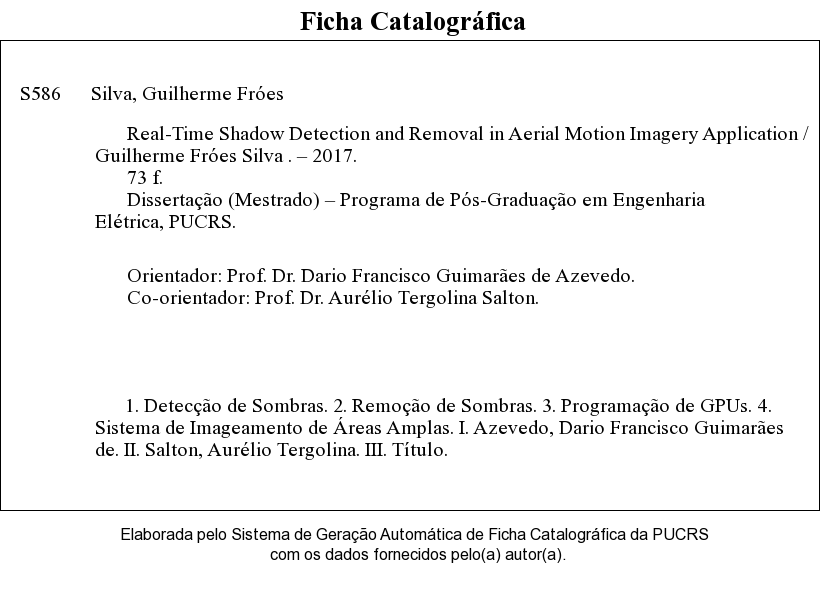
\includegraphics[width=\textwidth]{ficha_catalografica}
% \end{fichacatalografica}

%% EXEMPLO:
 \begin{fichacatalografica}
 	\vspace*{\fill}					% Posição vertical
 	\hrule							% Linha horizontal
 	\begin{center}					% Minipage Centralizado
 	\begin{minipage}[c]{12.5cm}		% Largura
	
 	\imprimirautor
	
 	\hspace{0.5cm} \imprimirtitulo  / \imprimirautor. --
 	\imprimirlocal, \imprimirdata-
	
 	\hspace{0.5cm} \pageref{LastPage} p. : il. (algumas color.) ; 30 cm.\\
	
 	\hspace{0.5cm} \imprimirorientadorRotulo~\imprimirorientador\\
 	\hspace{0.5cm} \imprimircoorientadorRotulo~\imprimircoorientador\\
	
 	\hspace{0.5cm}
 	\parbox[t]{\textwidth}{\imprimirtipotrabalho~--~\imprimirinstituicao,
 	\imprimirdata.}\\
	
 	\hspace{0.5cm}
 		1. Palavra chave 1.
 		2. Palavra chave 2.
 		I. \imprimirorientador.
 		II. \imprimircoorientador.
 		III. \imprimiruniversidade.
 		IV. \imprimirescola. \\	
	
 	\hspace{8.75cm} CDU 02:141:005.7\\
	
 	\end{minipage}
 	\end{center}
 	\hrule
 \end{fichacatalografica}

% ---
% Inserir errata
% ---
%\begin{errata}
%Elemento opcional da \citeonline[4.2.1.2]{NBR14724:2011}. Exemplo:
%
%\vspace{\onelineskip}
%
%FERRIGNO, C. R. A. \textbf{Tratamento de neoplasias ósseas apendiculares com
%reimplantação de enxerto ósseo autólogo autoclavado associado ao plasma
%rico em plaquetas}: estudo crítico na cirurgia de preservação de membro em
%cães. 2011. 128 f. Tese (Livre-Docência) - Faculdade de Medicina Veterinária e
%Zootecnia, Universidade de São Paulo, São Paulo, 2011.
%
%\begin{table}[htb]
%\center
%\footnotesize
%\begin{tabular}{|p{1.4cm}|p{1cm}|p{3cm}|p{3cm}|}
%  \hline
%   \textbf{Folha} & \textbf{Linha}  & \textbf{Onde se lê}  & \textbf{Leia-se}  \\
%    \hline
%    1 & 10 & auto-conclavo & autoconclavo\\
%   \hline
%\end{tabular}
%\end{table}
%
%\end{errata}
% ---

% ---
% Inserir folha de aprovação
% ---

% Isto é um exemplo de Folha de aprovação, elemento obrigatório da NBR
% 14724/2011 (seção 4.2.1.3). Você pode utilizar este modelo até a aprovação
% do trabalho. Após isso, substitua todo o conteúdo deste arquivo por uma
% imagem da página assinada pela banca com o comando abaixo:
%
% \includepdf{folhadeaprovacao.pdf}
%
 \begin{folhadeaprovacao}

   \begin{center}
     {\ABNTEXchapterfont\large\imprimirautor}

     \vspace*{\fill}\vspace*{\fill}
     {\ABNTEXchapterfont\bfseries\Large\imprimirtitulo}
     \vspace*{\fill}
    
     \hspace{.45\textwidth}
     \begin{minipage}{.5\textwidth}
         \imprimirpreambulo
     \end{minipage}%
     \vspace*{\fill}
    \end{center}
    
%    \vfill
    
    Aprovado: 

    \assinatura{\textbf{\imprimirorientador} \\ Orientador}
    \assinatura{\textbf{\imprimircoorientador} \\ Co-orientador}
    \assinatura{\textbf{Professor, Ph.D.}  \\ Universidade}
    %\assinatura{\textbf{Professor} \\ Convidado 3}
    %\assinatura{\textbf{Professor} \\ Convidado 4}
 	
 	\vfill
 	     
    \begin{center}
%     \vspace*{0.5cm}
     {\large\imprimirlocal}
     \par
     {\large\imprimirdata}
%     \vspace*{1cm}
   \end{center}
  
 \end{folhadeaprovacao}
% ---

% ---
% Dedicatória
% ---
\begin{dedicatoria}
   \vspace*{\fill}
   \centering
   \noindent
   \textit{ Aos meus pais, a quem serei eternamente grato. } \vspace*{\fill}
\end{dedicatoria}
% ---

% ---
% Agradecimentos
% ---
\begin{agradecimentos}

\blindtext

\blindtext

\end{agradecimentos}
% ---

% ---
% Epígrafe
% ---
\begin{epigrafe}
    \vspace*{\fill}
	\begin{flushright}
\textit{    
"All that is gold does not glitter \\
Not all those who wander are lost \\
% Not all those who wander are lost..." \\
The old that is strong does not wither \\
Deep roots are not reached by the frost \\
From the ashes a fire shall be woken \\
A light from the shadows shall spring \\
Renewed shall be blade that was broken \\
The crownless again shall be king" \\
}
    (J. R. R. Tolkien)
	\end{flushright}
\end{epigrafe}
% ---

% ---
% RESUMOS
% ---

% abstract
\begin{resumo}
 \blindtext

 \vspace{\onelineskip}
    
 \noindent
 \textbf{Palavras-chaves}: Palavra-chave 1. Palavra-chave 2.
\end{resumo}

% resumo em portugues
\begin{resumo}[Abstract]
 \begin{otherlanguage*}{english}
   \blindtext

   \vspace{\onelineskip}
 
   \noindent 
   \textbf{Key-words}: Key-word 1. Key-word 2. 
 \end{otherlanguage*}
\end{resumo}


% ---
% inserir lista de ilustrações
% ---
\pdfbookmark[0]{\listfigurename}{lof}
\listoffigures*
\cleardoublepage
% ---

% ---
% inserir lista de tabelas
% ---
\pdfbookmark[0]{\listtablename}{lot}
\listoftables*
\cleardoublepage
% ---

% ---
% inserir lista de abreviaturas e siglas
% ---

\begin{siglas}

    \item[CPU] Unidade Central de Processamento (do inglês, \textit{Central Processing Unit})
    \item[GPU] Unidade de Processamento Gráfico (do inglês, \textit{Graphics Processing Unit})

\end{siglas}
% ---

% ---
% inserir lista de símbolos
% ---
\begin{simbolos}
  %\item[$Q^{-1}$] Inversa da Função de Distribuição Acumulada

  \item[$\emptyset$] Empty set. In set theory, is a set which contains no elements
   
  \item[$\lambda$] Wavelength of the incident light

\cleardoublepage
   
\end{simbolos}
% ---

% ---
% inserir o sumario
% ---
\pdfbookmark[0]{\contentsname}{toc}
\tableofcontents*
\cleardoublepage
% ---


% ----------------------------------------------------------
% ELEMENTOS TEXTUAIS
% ----------------------------------------------------------
\textual

% Aqui é realizada a inclusão de arquivos no programa principal.
\chapter{Introdução}
\Blindtext

\section{Objetivos}

\section{Organização}%Structure

%%% REMOVER %%%
\section{\LaTeX ~super introdução}
Muito rapidamente, como usar o \LaTeX.

\subsection{Citações}
Para citar um autor, use o comando \verb|\cite{}| que gera $\rightarrow$ \cite{biswal1995}. 

Caso queira usar o nome do autor no texto, use \verb|\citeonline{}| que gera $\rightarrow$ \citeonline{biswal1995}.

% Este comando é do Abntex2
Para citações longas: \verb|\begin{citacao}...\end{citacao}| que gera:

\begin{citacao}
	'' \blindtext ``
\end{citacao}

\subsection{Figuras/Quadros/Tabelas}
A legenda em figuras, tabelas ou quadros, devem ficar por cima, enquanto a fonte fica por baixo. Exemplo na Figura \ref{f:ref-cruzada} abaixo:

% [H] é pra forçar a figura a aparecer logo abaixo do texto. Pesquise por "floats placement" para entender melhor.
\begin{figure}[H] 
	\centering % centralizando
	\caption{Exemplo de Figura}
	\includegraphics[draft]{teste.png}
	
	Fonte: \cite{Raichle2011}.
	\label{f:ref-cruzada}
\end{figure}
\chapter{Fundamentos Teóricos}
\Blindtext

% Capitulos seguintes, relativos ao desenvolvimento do trabalho em si
%\include{Desenvolvimento A}
\chapter{Desenvolvimento A}
\Blindtext
%\include{Desenvolvimento B}
\chapter{Desenvolvimento B}
\Blindtext
%\include{Desenvolvimento C}
\chapter{Desenvolvimento C}
\Blindtext

\chapter{Resultados}
%\chapter{Resultados e Discussão}
\Blindtext
\chapter{Conclusão}
\Blindtext


% ----------------------------------------------------------
% ELEMENTOS PÓS-TEXTUAIS
% ----------------------------------------------------------
\postextual


% ----------------------------------------------------------
% Referências bibliográficas
% ----------------------------------------------------------
\bibliography{refs}

% ----------------------------------------------------------
% Glossário
% ----------------------------------------------------------
%
% Consulte o manual da classe abntex2 para orientações sobre o glossário.
%
% \glossary

% ----------------------------------------------------------
% Apêndices
% ----------------------------------------------------------

% ---
% Inicia os apêndices
% ---
%\begin{apendicesenv}

% Imprime uma página indicando o início dos apêndices
%\partapendices


%\end{apendicesenv}
% ---


% ----------------------------------------------------------
% Anexos
% ----------------------------------------------------------

% ---
% Inicia os anexos
% ---
\setboolean{@twoside}{false}

% \begin{anexosenv}

% % Imprime uma página indicando o início dos anexos
% \partanexos
% \thispagestyle{plain}

% \end{anexosenv}

%---------------------------------------------------------------------
% INDICE REMISSIVO
%---------------------------------------------------------------------

\printindex

%%%%%%%%%%% CAPA PUCRS %%%%%%%%%%%%
\afterpage{%
	\newgeometry{a4paper,lmargin=0mm,rmargin=0mm,tmargin=0mm,bmargin=0mm}
	% material for this page
	\noindent
\includegraphics[width=\textwidth]{contracapa.png}
	\clearpage
	\restoregeometry
}
%%%%%%%%%%%%%%%%%%%%%%%%%%%%%%%%%%%

\end{document}
